%%%%%%%%%%%%%%%%%%%%%%%%%%%%%%%%%%%%%%%%%%%%%%%%%%%%%%%%%%%%%%%%%%%%%%%%%%%%%%%%
% reconstruction.tex:
%%%%%%%%%%%%%%%%%%%%%%%%%%%%%%%%%%%%%%%%%%%%%%%%%%%%%%%%%%%%%%%%%%%%%%%%%%%%%%%%
\chapter{Event Reconstruction}
\label{sec:reco_chapter}
%%%%%%%%%%%%%%%%%%%%%%%%%%%%%%%%%%%%%%%%%%%%%%%%%%%%%%%%%%%%%%%%%%%%%%%%%%%%%%%%

Electrons, muons and jets expected from \WR and \nul decays traversed multiple CMS sub-detectors, 
as shown in Figure \ref{fig:particleTrajectories}.  Their trajectories and energies were measured 
from charged particle tracks reconstructed by the silicon tracker, and energy deposits reconstructed 
by the calorimeters and the muon detectors.  The high energy of expected leptons and jets motivated 
the use of specific lepton and jet reconstruction algorithms described herein.

\begin{figure}[h]
	\centering
	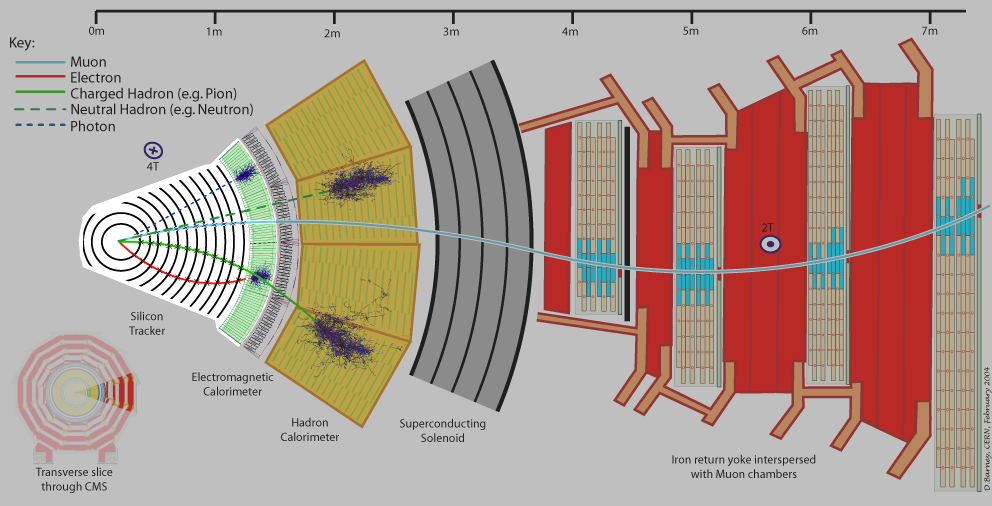
\includegraphics[width=0.75\textwidth]{figures/flowOfParticlesThroughCMS.png}
	\caption{Typical trajectories of particles travelling through CMS, from CERN.}
	\label{fig:particleTrajectories}
\end{figure}


\section{Electron Reconstruction}
\label{sec:eleReco}
Electrons ($e^{\pm}$) were the only particles from \WR decays expected to lose more than a few percent of their 
energy before reaching the ECAL.  One to two radiation lengths of material, depending on $\eta$, was in front of 
the ECAL \cite{ecalPerformanceInCollisions}, and about 35\% of electrons lose more than 70\% of their initial energy 
through bremsstrahlung before reaching the ECAL \cite{trackerPerformanceInCollisions}.  Bremsstrahlung photons were emitted in $\eta$ along their parent electron 
trajectories, but the magnetic field caused electrons to curve in $\phi$, and their photons were emitted a few 
degrees behind the $\phi$ positions were the electrons entered the ECAL.  The tracker did not detect these photons, 
but knowledge of electron bremsstrahlung was incorporated into a dedicated electron track reconstruction algorithm.  
This algorithm .


%RESUME HERE

They lost energy by emitting bremsstrahlung photons in $\phi$, which were detected 
by the ECAL.  A dedicated electron track algorithm reconstructed helical electron tracks from hits in tracker 
layers, and estimated the bremsstrahlung energy lost by comparing sequential hits.  The tracker measured 
electron $(\eta, \phi)$ trajectories, and the ECAL measured their energies including bremsstrahlung photons.

%THIS PARAGRAPH IS GOOD EXCEPT FOR THE QUESTION IN THE LAST SENTENCE ABOUT RECO ELECTRON POSITION
After traversing the tracker, electrons impinged on ECAL crystals and showered into lower energy $e^{\pm}$s.  
Electron energies were measured through the particle showers.  Approximately 94\% of an electron's energy coming 
into the ECAL was deposited over a 3 $\times$ 3 crystal area, but due to bremsstrahlung in the tracker an electron's 
total energy was deposited over a larger area.  To measure the total energy of each electron, ECAL energy deposits 
were reconstructed in superclusters (SCs) centered on the most energetic crystal, and were 3 or more crystals wide 
in $\eta$ depending on the electron shower shape.  SCs were 5 or more crystals wide in $\phi$, as shown in Figure 
\ref{fig:eleTrackAndSC}, to measure the energy lost by electrons through bremsstrahlung in the tracker.  Once a SC 
was reconstructed its $(\eta, \phi)$ position was calculated as the energy-weighted average position of all crystals 
in the SC, and this position was compared to $(\eta, \phi)$ trajectories of electron candidate tracks to identify 
an electron.  Each reconstructed electron was identified as a SC that geometrically matched at least one candidate 
track to within 1.1 degrees, about 60 crystals wide, in $\phi$, and within 0.004 units, less than $\frac{1}{2}$ a 
crystal wide, in $\eta$ \cite{ecalPerformanceInCollisions}.  Using the ECAL to determine reconstructed electron 
energies, the energy resolution for electrons from $Z \rightarrow ee$ decays with $\Et \approx 45$ $\GeV$ was better 
than 2\% for $|\eta| < 0.8$, and was between 2\% and 5\% elsewhere.  RECO ELECTRON POSITION?.

\begin{figure}[h]
	\centering
	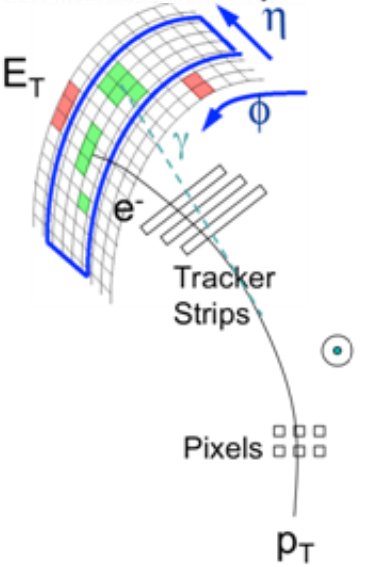
\includegraphics[width=0.75\textwidth]{figures/electronTrackAndSupercluster.png}
	\caption{The trajectory of a typical electron through the tracker and the ECAL.}
	\label{fig:eleTrackAndSC}
\end{figure}


\section{Muon Reconstruction}
\label{sec:muReco}
Muon ($\mu^{\pm}$) reconstruction started with reconstructing tracks in the silicon tracker.  Hits in individual 
tracker layers were reconstructed into helical tracks, and their $(\eta, \phi)$ trajectories determined reconstructed 
muon trajectories.  Muon momenta were measured through the curvature of reconstructed tracks, and were refined by muon 
detector measurements.

On average muons lost negligible energy before entering the muon detectors.  Hits in the muon chambers were reconstructed 
into helical tracks, and their radii of curvature were measured to improve the resolution of muon momenta measurements.  
Muon detector tracks were extrapolated back to the silicon tracker where the $(\eta, \phi)$ trajectories of silicon tracker 
and muon detector tracks were compared.  Each reconstructed muon was identified as a muon detector track whose trajectory 
matched a track in the silicon tracker.

The momentum of muons was determined using silicon tracker and muon detector measurements.  Four muon reconstruction 
algorithms fitted four continuous tracks \cite{cmsMuonRecoRunTwo} to silicon tracker and muon detector hits to estimate a 
muon's trajectory through CMS, represented in Figure \ref{fig:particleTrajectories}.  Each algorithm combined muon detector 
and silicon tracker measurements in a different way, and could exclude measurements with large uncertainty.  The quality 
of each continuous track was identified by a fit uncertainty $\chi^{2}/nDOF$ and momentum uncertainty $\sigma(\pt)/\pt$.  
The track with the lowest uncertainties was used to calculate the reconstructed muon momenta.  This procedure improved the 
momentum resolution for muons with $\pt > 200$ $\GeV$, which were expected in a significant fraction of $\WR \rightarrow \mu\mu jj$ 
events, as shown in Table \ref{tab:wrHighPtMuons}.

\begin{table}[h]
	\caption{Fraction of expected $\WR \rightarrow \mu\mu jj$ events that had at least one muon with $\pt > 200$ $\GeV$. 
	($\mnul = \frac{1}{2}\mWR$)}
	\label{tab:wrHighPtMuons}
	\centering
	\begin{tabular}{c|c}
		\mWR ($\TeV$) & Fraction of events with at least one high-$\pt$ muon (\%) \\  \hline
		1.0 &  80.  \\
		2.0 &  95.  \\ 
		3.0 &  98.  \\ \hline
	\end{tabular}
\end{table}


\section{Jet Reconstruction}
\label{sec:jetReco}
Through hadronization, photon radiation, and leptonic weak decays, quarks produced jets of photons, hadrons, and leptons.  Jet 
reconstruction began by reconstructing photons, electrons and muons, and charged and neutral hadrons.  Each charged hadron was 
reconstructed in a similar way to electrons, by geometrically matching an energy measured in an HCAL tower to a reconstructed 
track.  A charged hadron could also contain an ECAL SC if the SC $(\eta, \phi)$ position matched the HCAL tower.  Each neutral 
hadron was reconstructed as an HCAL tower, possibly associated with an ECAL SC, whose $(\eta, \phi)$ position did not match any 
reconstructed track.  Similarly, each photon was reconstructed as an ECAL SC whose position did not match any reconstructed track.  
After reconstructing individual particles, jets were reconstructed as clusters of individual particles, as shown in Figure 
\ref{fig:jetClustering}.

\begin{figure}[h]
	\centering
	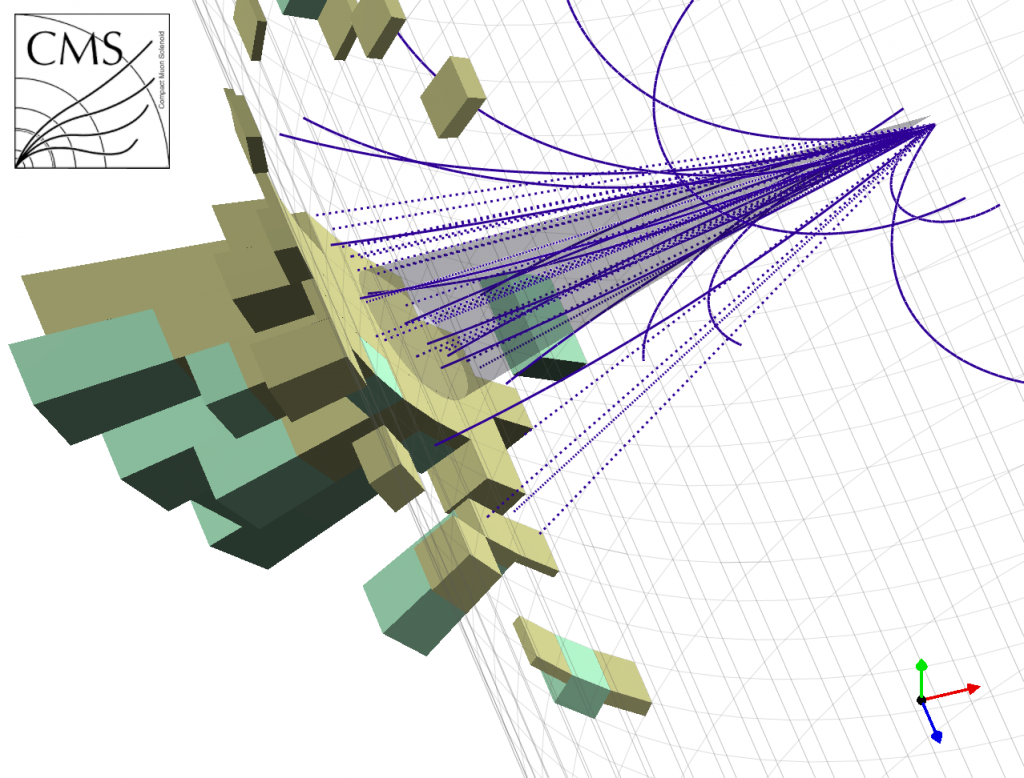
\includegraphics[width=0.75\textwidth]{figures/jetClusteringInCMS.png}
	\caption{A cone of reconstructed particles clustered into a jet, with the reconstructed vertex on the right.  
	From the CMS Experiment.}
	\label{fig:jetClustering}
\end{figure}

In each collision event, every reconstructed particle was considered a jet candidate, except charged hadrons that did not come 
from the reconstructed vertex with the highest $\sum \pt$.  Using the anti-$k_{T}$ algorithm \cite{antikt}, reconstructed particles 
were clustered into jets, each approximately $\Delta R = 0.4$ wide, based on their individual energies and trajectories.  Each jet's 
energy was the total energies of all constituents, and its $(\eta, \phi)$ trajectory was the energy-weighted average trajectory of 
all its constituents.


\section{Conclusion}
\label{sec:recoConclusion}
Energetic electrons, muons and jets produced in collisions were reconstructed using several CMS sub-detectors and high energy 
reconstruction algorithms.  Additional selections were applied to reconstructed leptons and jets to increase sensitivity to the \WR 
signal relative to ST processes that produced $\ell\ell jj$ events.

%%%%%%%%%%%%%%%%%%%%%%%%%%%%%%%%%%%%%%%%%%%%%%%%%%%%%%%%%%%%%%%%%%%%%%%%%%%%%%%%
